\section{Zielsetzung}
\label{sec:Zielsetzung}
Ziel des Versuch ist es die Zeeman-Aufspaltung von Spektrallinien genauer zu untersuchen.
Dazu wird ein Cd-Lampe mit einem Magnetfeld durchsetzt, damit sich die Energieniveaus aufspalten.

\section{Theorie}
\label{sec:Theorie}
\subsection{Quantenmechanische Grundlagen}
\label{sec:qm}
Aus der Quantenmechanik ist bekannt, dass das Atom aus einem Kern und einer Atomhülle besteht.
In der Atomhülle bewegen sich die Elektronen auf festen Energieniveaus.
Für Atome mit kleiner Kernladungszahl koppeln die einzelnen Bahndrehimpulse der Elektronen $\vec{l_\text{i}}$
zum Gesamtbahndrehimpuls
\begin{equation*}
    \vec{L} = \sum{\vec{l_\text{i}}}
\end{equation*} 
zusammen. Analoges geschieht für den Spin $s_\text{i}$ der Elektronen, dabei
müssen in beiden Fällen nur teilweise gefüllte Schalen beachtet werden, da sich bei vollen Schalen sie sich
jeweil zu $\vec{0}$ ergeben.
Aus dem Bahndrehimpuls der Elektronen $\vec{L}$ und dem Spin der Elektronen $\vec{S}$ ergibt sich der
Gesamtdrehimpulses $\vec{J} = \vec{L} + \vec{S}$, solange das Atom nicht von einem starken Magnetfeld durchsetzt wird.
Zu jedem Drehimpuls gehört auch ein magnetisches Moment.
Dabei ergibt sich das magnetische Moment für den Gesamtdrehimpuls 
\begin{equation*}
  \vec{\mu_\text{J}} = \vec{\mu_\text{L}} + \vec{\mu_\text{S}}
\end{equation*}
aus der Summe der magnetischen Momente für Spin 
\begin{equation}
\label{eqn:magspin}
  \vec{\mu_\text{S}} = -g_\text{S} \mu_\text{B} \vec{S}
\end{equation}
und Bahndrehimpuls
\begin{equation}
  \label{ean:magbahn}
  \vec{\mu_\text{L}} = - \mu_\text{B} \vec{L}.
\end{equation}
Mit dem Betrag eines jeden Drehimpulses $|\vec{L'}| = \sqrt{L' \left(L'+1\right)}$ ergibt sich somit
\begin{equation}
  \label{eqn:gj}
  g_\text{J} = \frac{\num{3.0023}J(J+1)+\num{1.0023}[S(S+1)-L(L+1)]}{2J(J+1)},
\end{equation}
dabei wird $g_\text{S} = \num{2.00232}$ verwendet.
Die Kennzeichnung der Schalen lassen sich durch \ce{^{2S+1}L_J} ausdrücken, wobei für $L$ Buchstaben anstelle
von Zahlen verwendet. So entspricht eine Schale mit $L=0, S=1, J=1$ dem Ausruck \ce{^3S_1}.
% Für Atome mit sehr großer Kernladungszahl ist die direkte Kopplung zwischen Bahndrehimpuls des einzelnen
% Elektrons mit seinem Spin größer als die Kopplung untereinander. Sie koppeln zum Gesamtbahndrehimpuls der Atomhülle
% anders als bisher, dabei ergeben sich ausden einzelnen Gesamtbahndrehimpulse 
% \vec{j_\text{i}}=\vec{l_\text{i}}+\vec{s_\text{i}}, der Gesamtbahndrehimpuls der Atomhülle 
% \begin{equation*}
%     \vec{J_\text{i}}=\sum{\vec{j_\text{i}}}.
% \end{equation*}

\subsection{Verhalten eines Atoms im Magnetfeld}
\label{sec:mag}
Wird nun ein äußeres Magnetfeld $\vec{B}$ angelegt, so spalten sich die Energieniveaus in $2J+1$ Unterniveaus auf.
Dies hat seine Ursache in der Wechselwirkung des magnetischen Moments mit dem Magnetfeld und der Richtunsquantelung.
Bekanntlich präzidiert $\vec{\mu_\text{J}}$ um die Feldrichtung des äußeren Magnetfeldes und der senkrechte Anteil mittelt 
sich herraus. Für die $z$-Komponete ergibt sich mit der Richtungsquantelung die Wechselwirkungsenergie zu
\begin{equation}
  \label{eqn:nzee}
  E_\text{magn} = m_\text{J} g_\text{J} \mu_\text{B} |\vec{B}|,
\end{equation}
mit der Orientierungsquantenzahl $m_\text{J} = -J, \ldots, J-1 ,J$. Dieser Effekt ist besser bekannt unter
dem Namen normalem Zeeman-Effekt und gilt für Fall, dass der Spin verschwindet.
Besitzt die Atomhülle eine nicht verschwindenen Spinanateil $\vec{S} \neq \vec{0}$, dann Spalten 
die Niveaus nicht mehr in äquidistante Unterniveaus auf, sondern es gibt eine Energieverschiebung nach
\begin{equation}
    \label{eqn:azee}
    E_\text{mag} = [m_\text{\alpha} \cdot g(L_\text{\alpha}, S_\text{\alpha}, J_\text{\alpha}) - m_\text{\beta} g(L_\text{\beta}, S_\text{\beta}, J_\text{\beta})] \text{\mu_B} B.
\end{equation}

\subsection{Optische Übergänge}
\label{sec:opt}
In der Quantenmechanik lassen sich Bedingungen für optische Übergänge herleiten, dabei ergibt sich die Auswahlregel
\begin{equation*}
    m_\text{J} = \pm 1, 0.
\end{equation*}
Für einen Übergang aus dem Niveau mit Energie $E__\text{\alpha}$ in ein Niveau mit Energie $E_\text{\beta}$ muss
ein Photon der Frequenz
\begin{equation}
    \label{eqn:freq}
    \mu_\text{\alpha\beta} = \frac{E_\text{\alpha}-E_\text{\beta}}{h} 
\end{equation}
absorbiert beziehungsweise emittiert werden.
Die Polarisation des ausgesendeten Lichts hängt mit der Änderung der Orientierungsquantenzahl ab.
So wird bei einem Übergang mit $\Delta m_\text{J} = 0$ linear-polarisiertes Licht frei, mit Schwingungsrichtung
parallel zur Feldrichtung. Dieser Übergang wird auch als \pi-Übergang bezeichnet, während ein Übergang mit
$\Delta m_\text{J} = \pm 1$ als \sigma-Übergang bezeichnet wird. Dieser Übergang strahl in Feldrichtung
zirkular-polarisiertes Licht aus, welches sich in seinem Drehsinn unterscheidet. Senkrecht zum erscheint das 
Licht also linear-polarisiert. Ein Beispiel zu so einem Übergang ist in Abbildung \ref{fig:aufspaltung} dargestellt.
Für den normalen Zeeman-Effekt ergibt sich also eine Aufspaltung einer Spektrallinie in drei Spektrallinien, 
denn die Niveaus spalten ja äquidistant auf und somit entsendet eine Gruppe von erlaubten Übergängen
mit gleichem $\Delta m_\text{J}$, also gleicher Energiedifferenz, Quanten gleicher Frequenz.

\begin{figure}[htb]
  \centering
  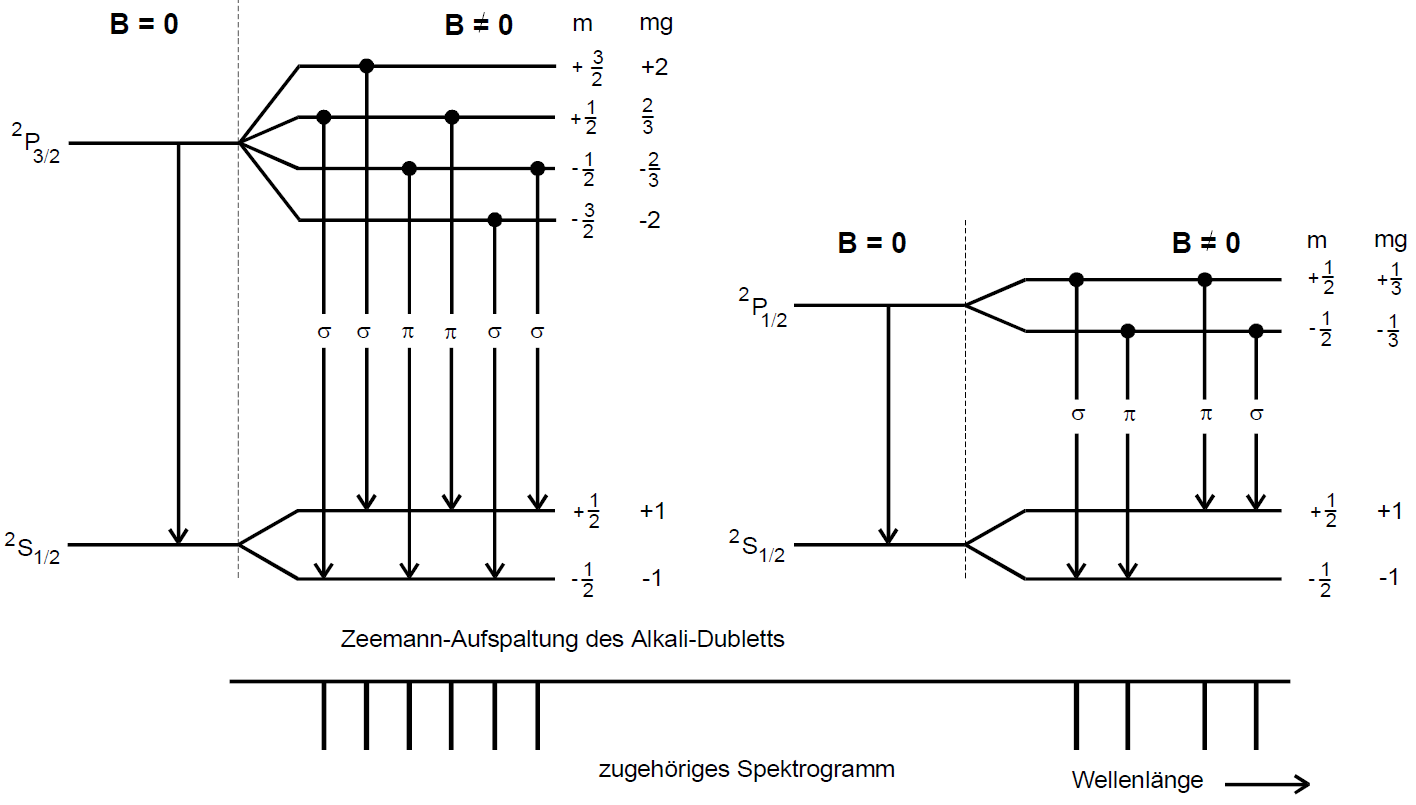
\includegraphics[height=5.5cm]{content/pictures/Aufspaltung.png}
  \caption{Die Energieniveaus-Aufspaltung für den anormalen Zeeman-Effekt. \cite{anleitung_alt}}
  \label{fig:aufspaltung}
\end{figure}
\FloatBarrier